\section{Background}

\subsection{A brief introduction to boolean networks}

Random Boolean Networks, also known as Kaffman networks, were originally developed as a model of genetic regulatory networks \cite{kauffman1969metabolic}.
The model makes no assumptions about the actual functioning of the nodes in the network,
making them useful to model a wide range of phenomena.
The simplification of a system to a boolean model doesn't pose a problem,
as any multi-valued network can be transformed to a corresponding binary one.

A RBN is usually described by its number of nodes $N$ and the in-degree $K$ of the nodes,
that is, how many nodes each node depends on (also known as its ancestors).
RBNs can have both homogenous and heterogenous in-degrees.
In heterogenous networks, one usually describes the average connectivity $<K>$ instead.

Each node can have a state of zero or one.
The next state of the node is solely determined by the current combination of states of its ancestors.
Each combination leads to a new state of zero or one,
with the probability given by a binomial distribution usually having $<p>=0.5$.
Figure \ref{figure:sample-homogenous-rbn} visualizes a homogenous RBN with N=3 K=2, and P=0.5.

\begin{figure}
  \centering
  \subfloat[RBN topology]{
    \begin{tikzpicture}
      \node[vertex] (a) {a};
      \node[vertex] (b) [below left of=a] {b};
      \node[vertex] (c) [below right of=a] {c};

      \draw[edge] (a) to[bend right] (b);
      \draw[edge] (a) to (c);

      \draw[edge] (b) to (a);
      \draw[edge] (b) to[bend right] (c);

      \draw[edge] (c) to[bend right] (a);
      \draw[edge] (c) to (b);
    \end{tikzpicture}
  }
  \subfloat[Transition table for node a]{
    \begin{tabular}[b]{ c c | c}
      \multicolumn{2}{c}{Ancestor states} & New state \\
      \hline
      0 & 0 & 0 \\
      0 & 1 & 1 \\
      1 & 0 & 0 \\
      1 & 1 & 1 \\
    \end{tabular}
  }
  \caption{An example homogenous RBN with N=3, K=2.}
  \label{figure:sample-homogenous-rbn}
\end{figure}

In the classical RBN model (CRBN), all nodes update at the same time,
therefore the states of the network at $t+1$ only depends on the states at $t$.
This is a simplification that isn't quite accurate for all systems,
notably gene regulation networks where the system doesn't operate in lockstep.
There are therefore a number of updating schemes on the spectrum of determinism and randomness.

The dynamics of an RBN can be categorized as being in either the ordered, critical, or chaotic phase.
These phases can be identified by how large a part of the network state is able to change over time,
whether similar states tend to converge or diverge over time,
and the networks resistance to perturbations (outside changes to the network).

As these phases are easy to identify visually,
we will plot the states of the RBN in a square lattice,
with the network states plotted horizontally, and time flowing downwards.
A node is drawn as white if its state is one, black otherwise.
The phases are visualized in figure \ref{figure:rbn-phases}.

\begin{figure}
  \subfloat[Ordered phase, K=1]{
    
\includegraphics[width=0.3\columnwidth]{background/ordered-phase.pdf}
    \label{figure:rbn-ordered}
  }
  \subfloat[Critical phase, K=2]{
    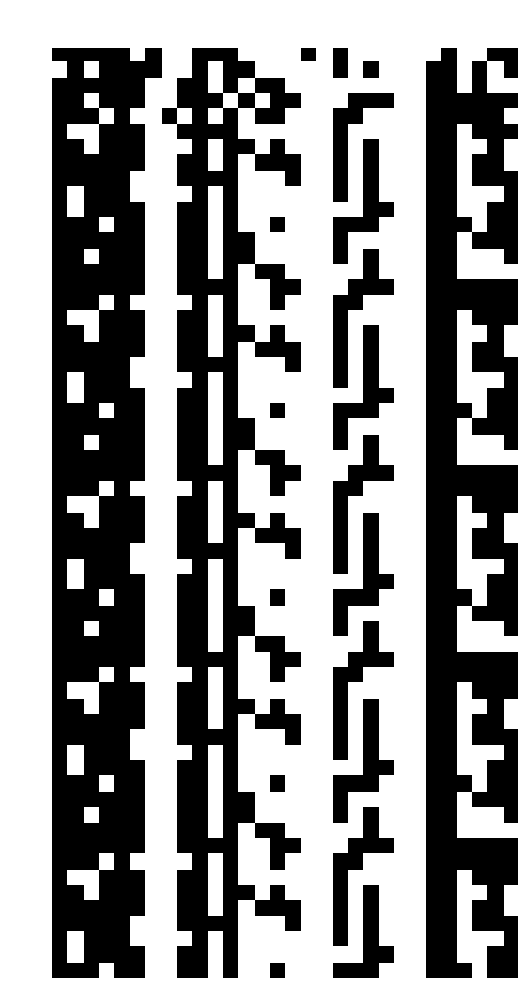
\includegraphics[width=0.3\columnwidth]{background/critical-phase.pdf}
    \label{figure:rbn-critical}
  }
  \subfloat[Chaotic phase, K=3]{
    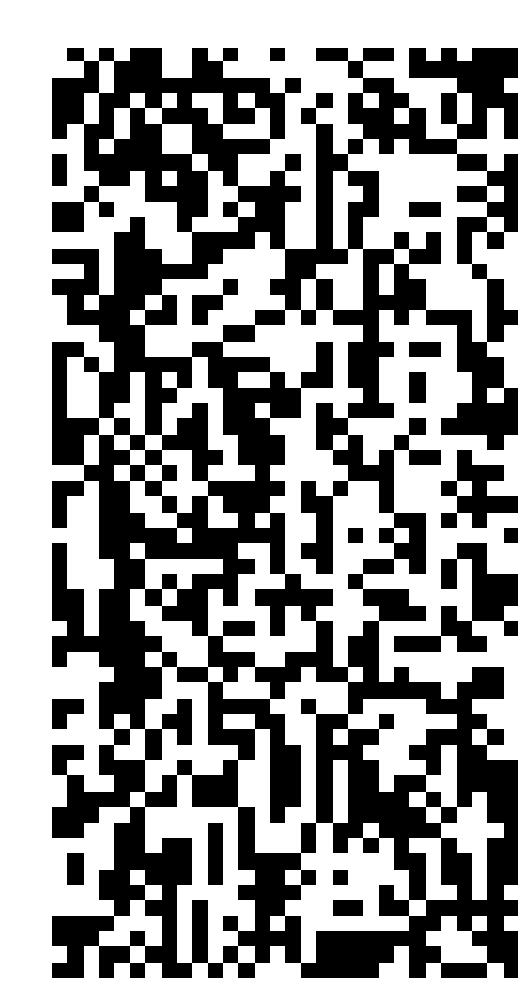
\includegraphics[width=0.3\columnwidth]{background/chaotic-phase.pdf}
    \label{figure:rbn-chaotic}
  }

  \caption{Trajectories through state-space for RBNs with $N=30, K=[1,2,3]$, visualizing the different phases.}
  \label{figure:rbn-phases}
\end{figure}

In general, RBNs in the critical phase are the most interesting.
These are seemingly able to support both information transmission, storage and modification,
capacities required for computation \cite{langton3computation}.
Critical systems are found on the edge of chaos, on the phase transition between ordered and chaotic networks.
For classical RBNs with $<p>=0.5$, critical networks are usually found at $<K>=2$ \cite{gershenson2004introduction},
although one could still create networks with similar dynamics for different $K$.

A more thorough introduction to RBNs is available in \cite{gershenson2004introduction}.

\subsection{Using boolean networks in reservoir computing}

Can we use these simple networks for computation?
Turns out Yes!, as shown in this paper \cite{rbn-reservoir}, and it works reasonably well.

Takeaways from the paper:
\begin{itemize}
  \item Relationship between dynamical properties and computational power
  \item Required connections to input layer, how much perturbation required?
\end{itemize}

Advantages include being MUCH less complex than Echo-state networks and similar, as those require operations such as 'multiplication' which is orders more complex than the simple lookup-table transitions for the RBN nodes.


\begin{itemize}
  \item LSM / ESN
  \item 2013-RBN Paper
  \item RBN-Kauffmann networks
  \item Sipper programming complexity (Fra TDT1/22) Snakk om vanskeligheten av å programmere
\end{itemize}
